\documentclass{scrartcl}			% defines the kind of document you want to produce

% Include different packages:
\usepackage[utf8]{inputenc}
\usepackage[T1]{fontenc}
\usepackage{lmodern}
\usepackage[english]{babel}
\usepackage{amsmath}
\usepackage{float}
\usepackage{graphicx}           	% include graphics
\usepackage{caption}
\usepackage{subcaption}
\usepackage{hyperref}
\usepackage{listings}
\usepackage{fancyvrb}

\title{Neuroprothetik Exercise 3 \\
	Mathematical Basics 2}

\author{Aleksandra Teska}
\date{29. May 2018}


\begin{document} 					% Document begins here

\maketitle

\section{Implementation of following functions}		% start a new section
Following methods were implemented as functions in Python:
\begin{itemize}
	\item Forward (Explicit) Euler
	\item Heun Method
	\item Exponential Euler
\end{itemize}

\section{Solve Functions}		% start a new section

This exercise contain solving differential equation:

\begin{align}
\frac{dV}{dt} =  1 - V - t
\end{align}			
where $V(t = -4.5) = V_{0} = 04$ with the, solvers implemented above. Vary the step size $(1s, 0.5s, 0.1s, 0.012)$ and plot the results.\\
Plots can be found in section 4 on \ref{subsec_fig1_1}, \ref{subsec_fig1_2}, \ref{subsec_fig1_3}\\

Based on the plots we can notice the impact of the chosen step-size. As suggested, the resulted error of numerical approximation depends on the incremental step size. One can notice that with the biggest step size of 1s the suggested solutions overshoots/undershoots the desired solution.\\

Using a very small step size would be computationally problematic and also time costly. Additionally with a very small time step, the accumulated step error of $ \Detla $ t gets squared.

\newpage

\section{The Leaky Integrate and Fire Neuron}

The goal of this exercise was to implement a model of the leaky integrate and fire neuron. The following implementation was used:

\begin{Verbatim}[tabsize=4]
def LIFsin(T, dt, I):
	Cm = 1e-6
	g_leak = 100e-6
	V_rest  = -60e-3
	V_thr   = -20e-3
	V_spike = 20e-3

	t = np.linspace(0, T, int(T/dt))
	V = np.zeros(len(Isin))
	V[0] = V_rest

	for n in np.arange(0, len(Isin)-1):
		if   (V[n] < V_thr):
			V[n+1] = V[n] + dt/Cm * (-g_leak * (V[n] - V_rest) + I[n])
		elif (V[n] == V_spike):
			V[n+1] = V_rest
		elif (V[n] >= V_thr):
			V[n+1] = V_spike
	return V, t
\end{Verbatim}

Given following parameters:
\begin{itemize}
	\item $g_{leak}$ = 100 $\mu$S
	\item $V_{rest}$ = -60 mV
\end{itemize}

And simulate the cell for 50 ms ($\Delta t = 25 \mu s$ should be sufficient) with the following
current inputs:
\begin{itemize}
	\item constant 10 $\mu$A
	\item constant 20 $\mu$A
	\item rectified 50Hz sinus with 10 $\mu$A amplitude
	\item rectified 50Hz sinus with 30 $\mu$A amplitude
\end{itemize}

\newpage
\subsection{Results interpretation}

On the plots we can notice the spiking behavior of implemented integrated fire neuron. With this kind of implementation, the spike and reset of the potential value are happening almost instantaneously (within 2 $\Delta$t), without any hyperpolarizaton.\\

Additionally, we can notice differences in between each simulation. with stimulation of 10 $\mu$A reaching the threshold value of potential takes around 5 ms, while for the same stimulus with an amplitude of 20 $\mu$A the needed time a bit shorter then 2.5 ms.\\

When the input was changed to sinusoidal wave with frequency of 50 Hz, we can notice that also the responses are happening with the given frequency. With lower amplitude of that signal, we can see one spike in each period of the sinusoidal wave. For higher amplitude of 30 $\mu$A, we can observe multiple spikes.

\section{Plots}
\subsection{Plots of functions implemented in section 1}
\begin{figure}[hbpt!]					%start figure-environment
	\begin{flushleft}
		\hspace*{-0.7in}
		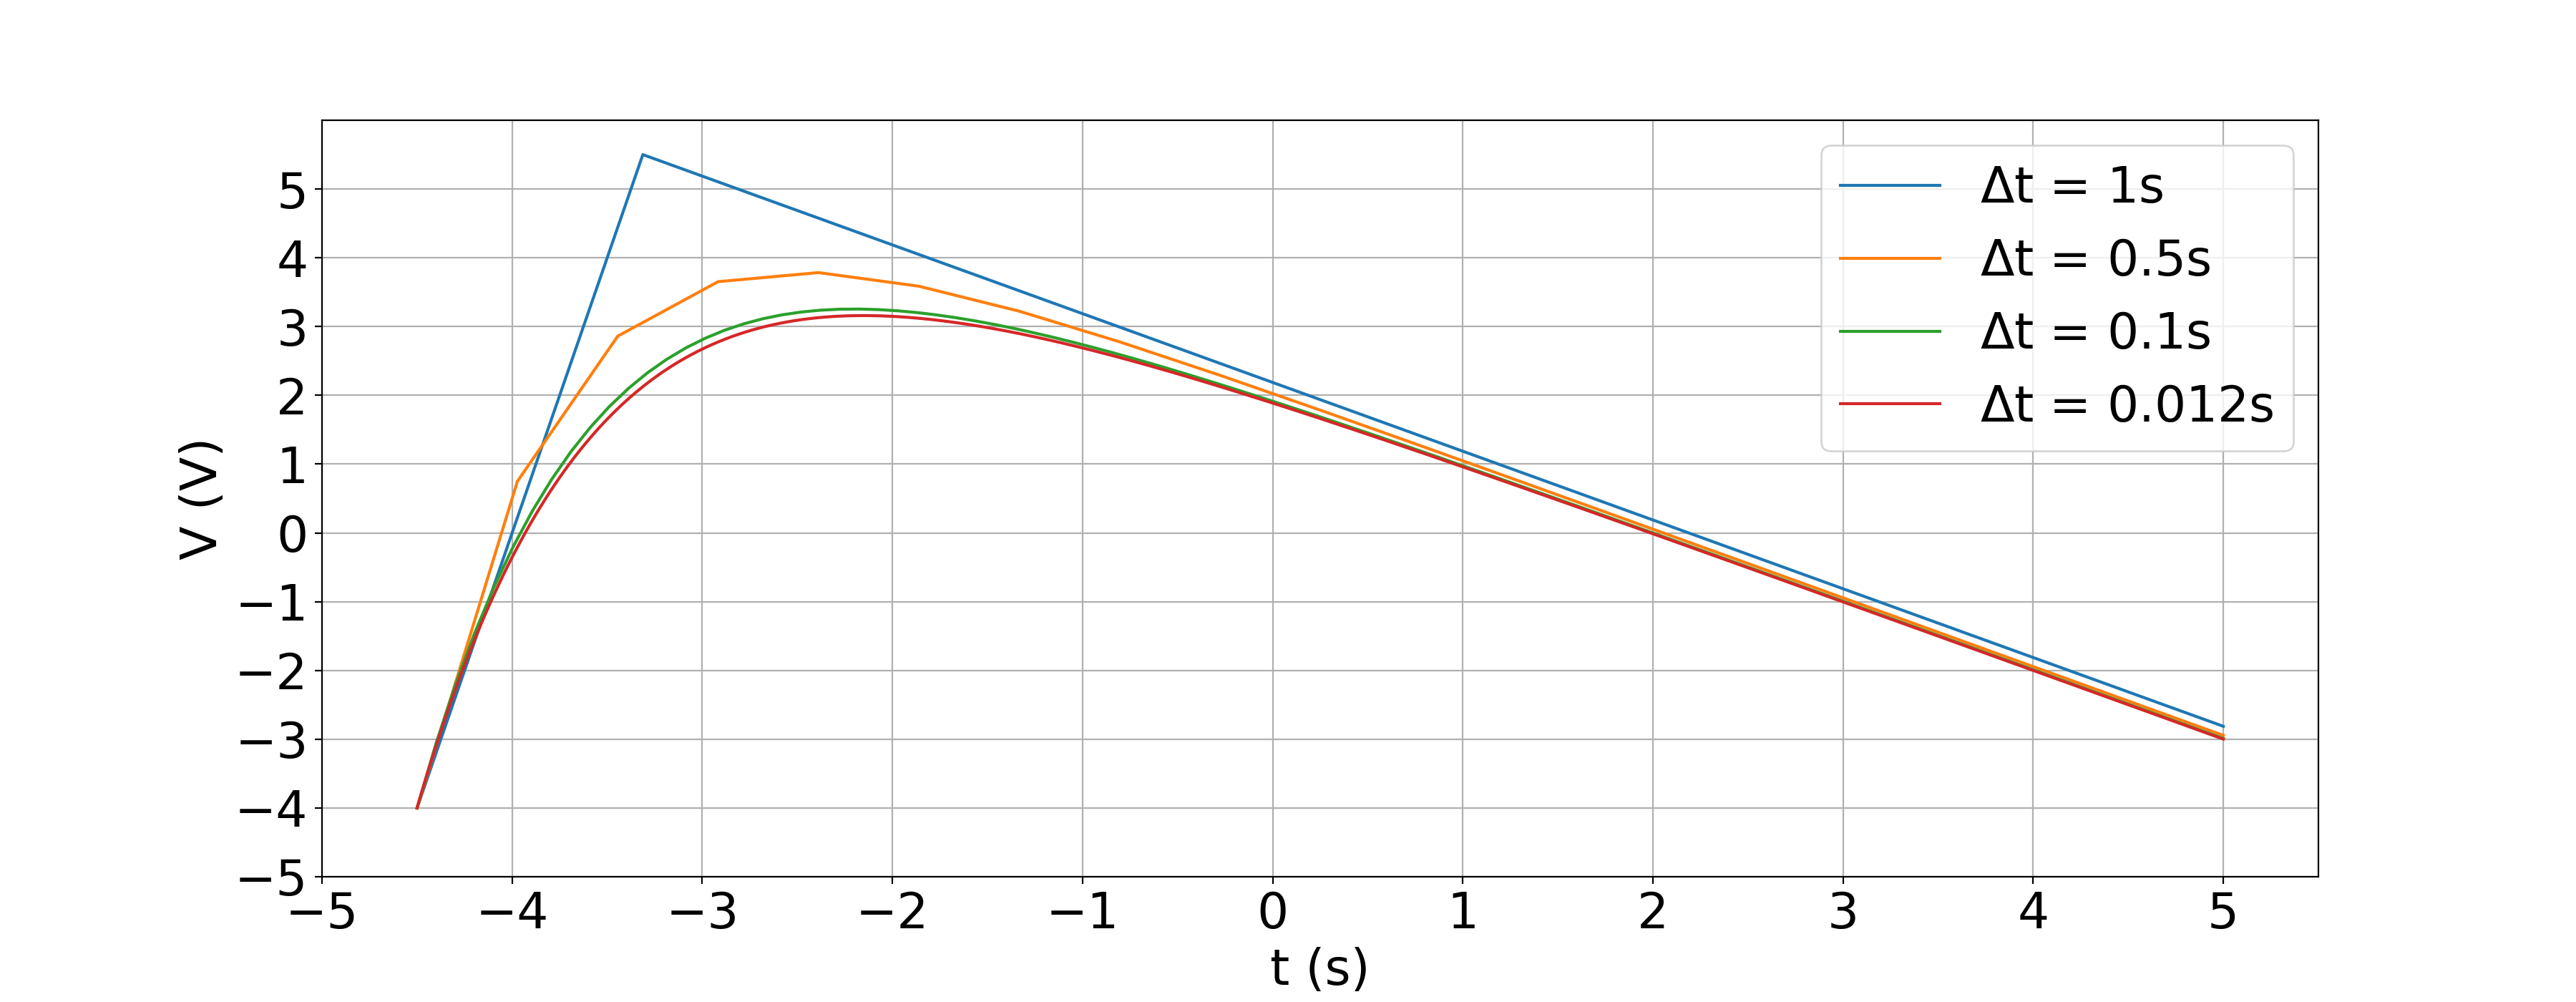
\includegraphics[scale=0.4]{1_1.png}
		\captionsetup{width=\linewidth}  %choose the with of the caption
		\caption{Approximations of the given differential equation in 2 with different methods and different step sizes Forward-Euler-Method. The different colors resemble the given timesteps visible in the legend.}
		\label{subsec_fig1_1} %choose a label, see subsection references
	\end{flushleft}
\end{figure}
\hspace*{0in}

\newpage
\begin{figure}[hbpt!]					%start figure-environment
	 \begin{flushleft}
		\hspace*{-0.7in}
		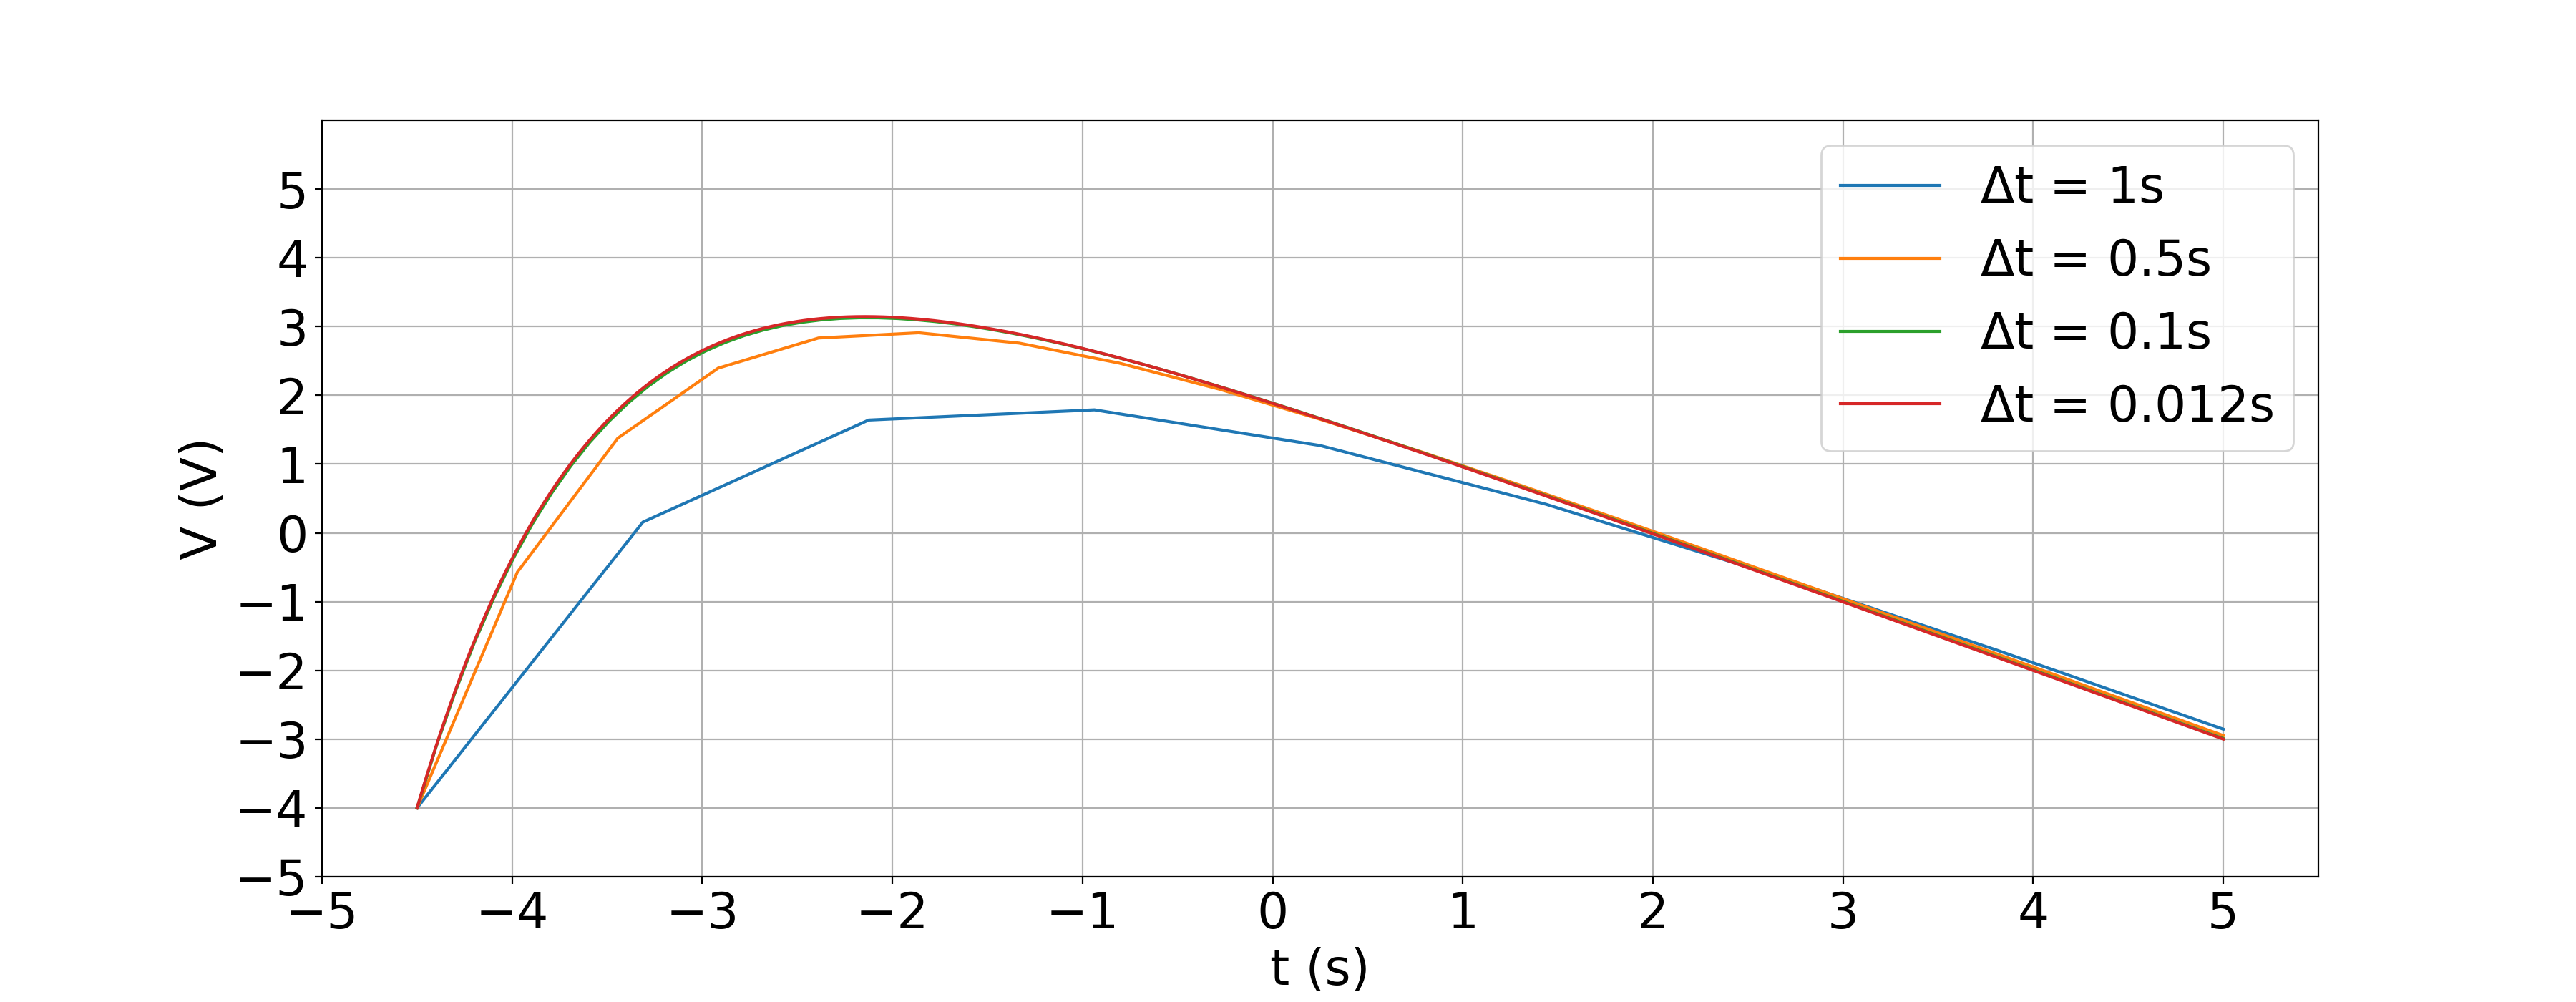
\includegraphics[scale=0.4]{1_2.png}
		\captionsetup{width=\linewidth}  %choose the with of the caption
		\caption{Approximations of the given differential equation in 2 with different methods and different step sizes Heun-Method.The different colors resemble the given timesteps visible in the legend.}
		\label{subsec_fig1_2} %choose a label, see subsection references
	\end{flushleft}
\end{figure}

\begin{figure}[hbpt!]					%start figure-environment
	 \begin{flushleft}
		\hspace*{-0.7in}
		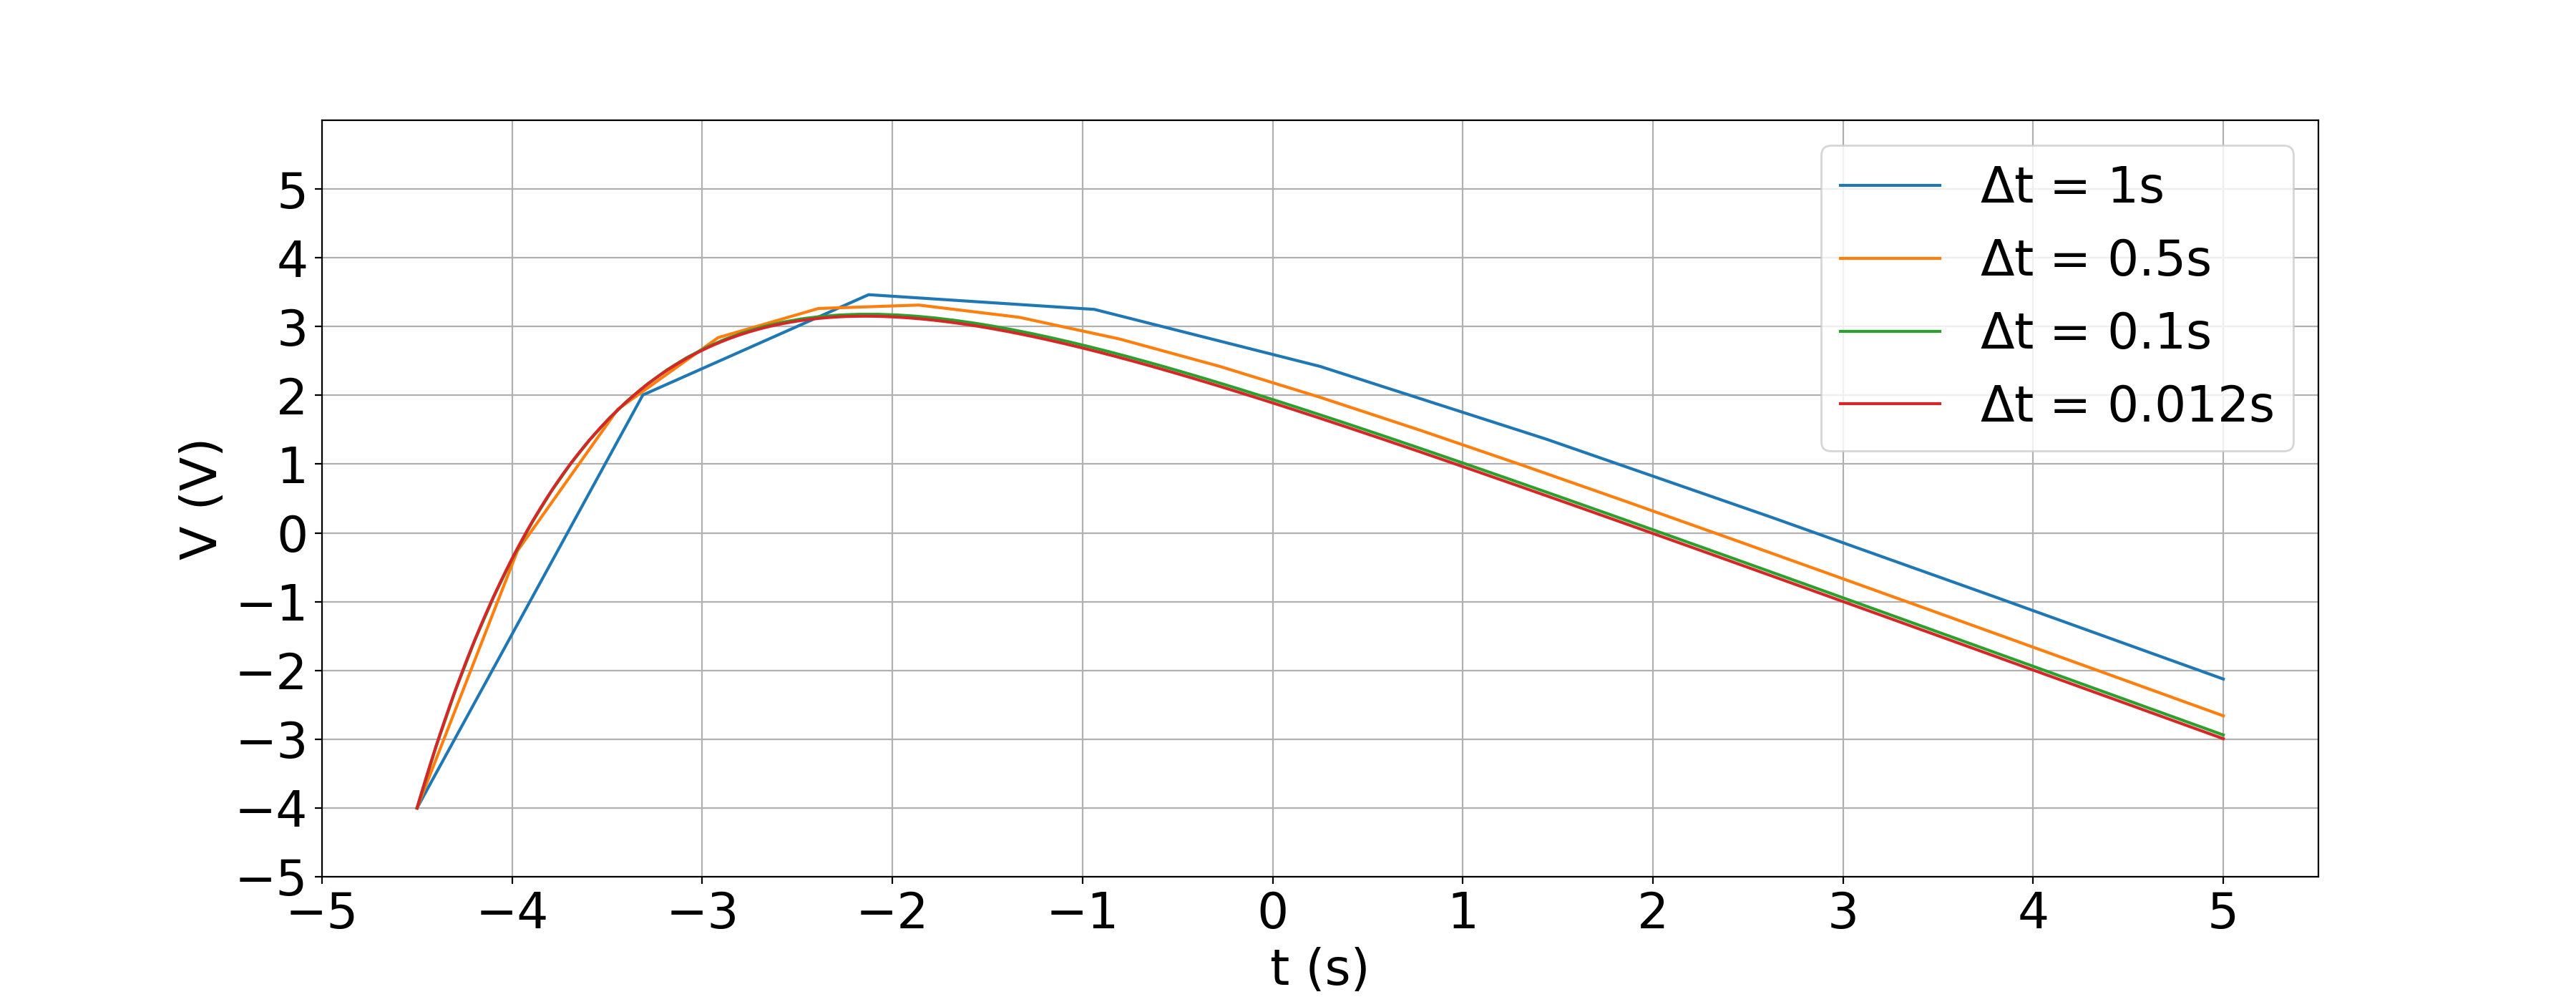
\includegraphics[scale=0.4]{1_3.png}
		\captionsetup{width=\linewidth}  %choose the with of the caption
		\caption{Approximations of the given differential equation in 2 with different methods and different step sizes Exponential-Euler Method. The different colors resemble the given timesteps visible in the legend.}
		\label{subsec_fig1_3} %choose a label, see subsection references
	 \end{flushleft}
\end{figure}


\newpage
\subsection{Plots of the rectified 50 Hz sinusoidal input}
\begin{figure*}[hbpt!]					%start figure-environment
	\centering
	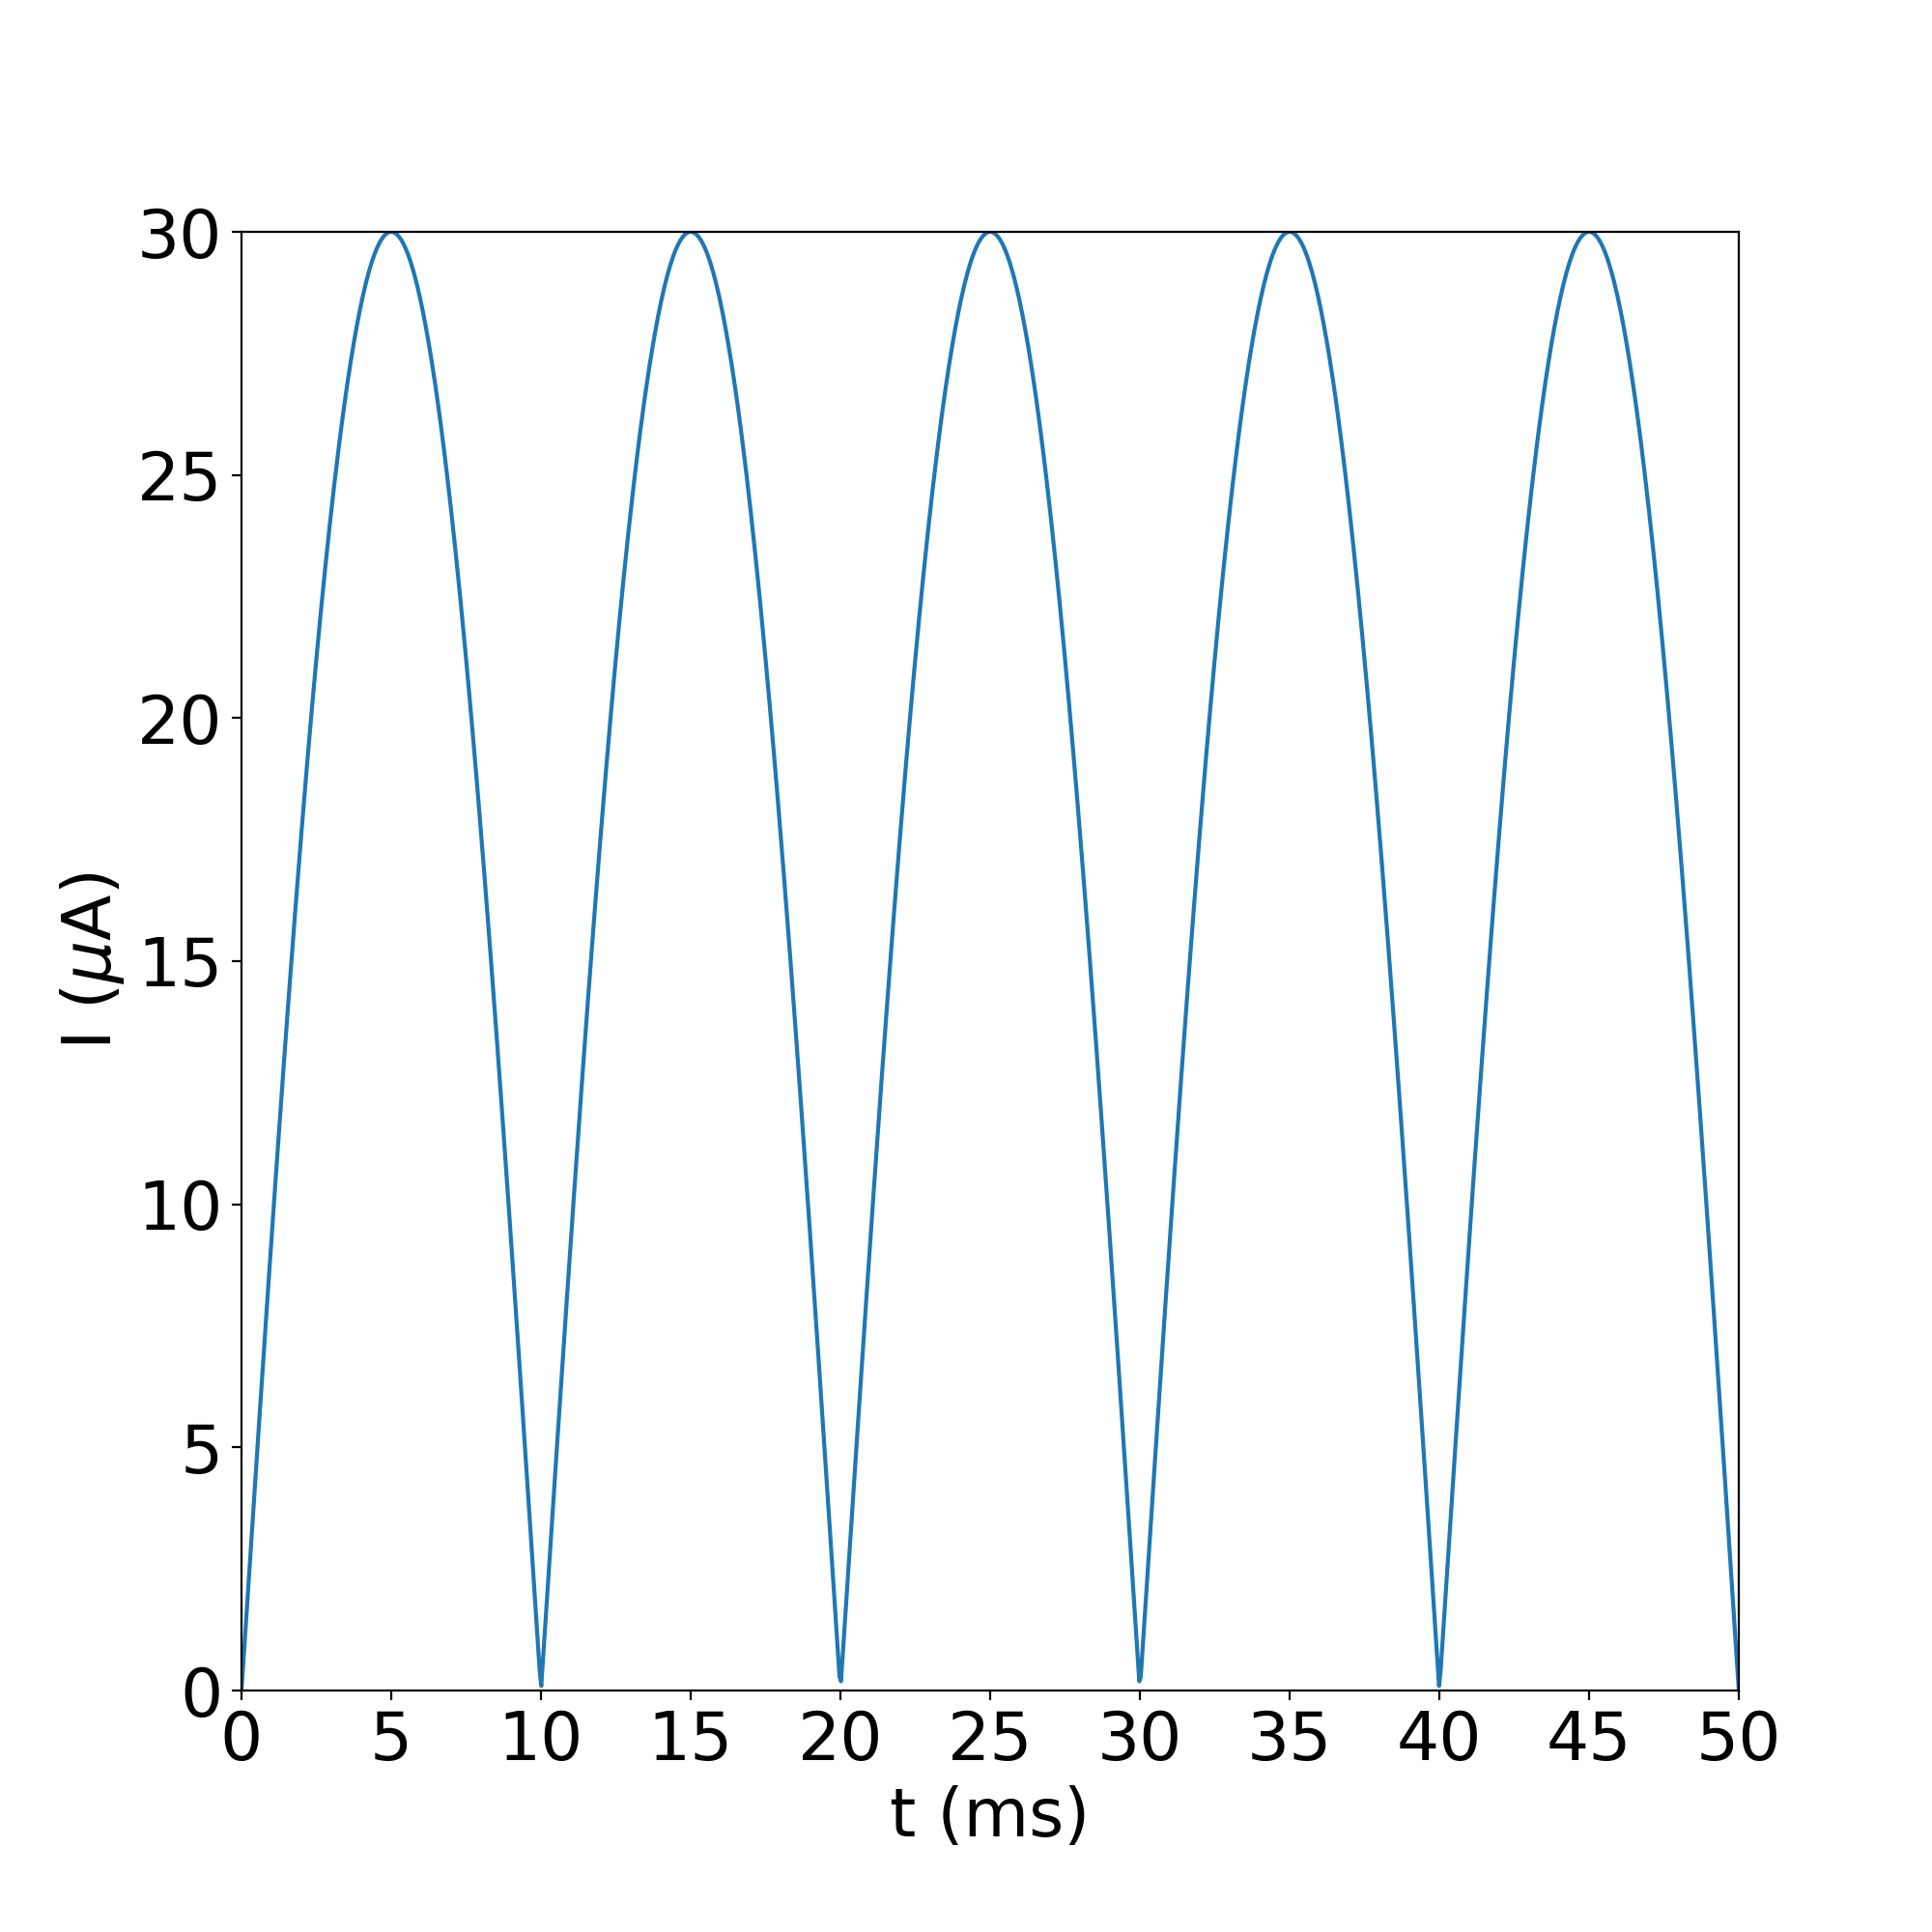
\includegraphics[scale=0.33]{2_1.png}
	\captionsetup{width=\linewidth}  %choose the with of the caption
	\caption{Rectified Sine with an amplitude of 10 $\mu$A for the model visible in Figure 8}
	\label{subsec_fig2_0} %choose a label, see subsection references
\end{figure*}

\begin{figure*}[hbpt!]					%start figure-environment
	\centering
	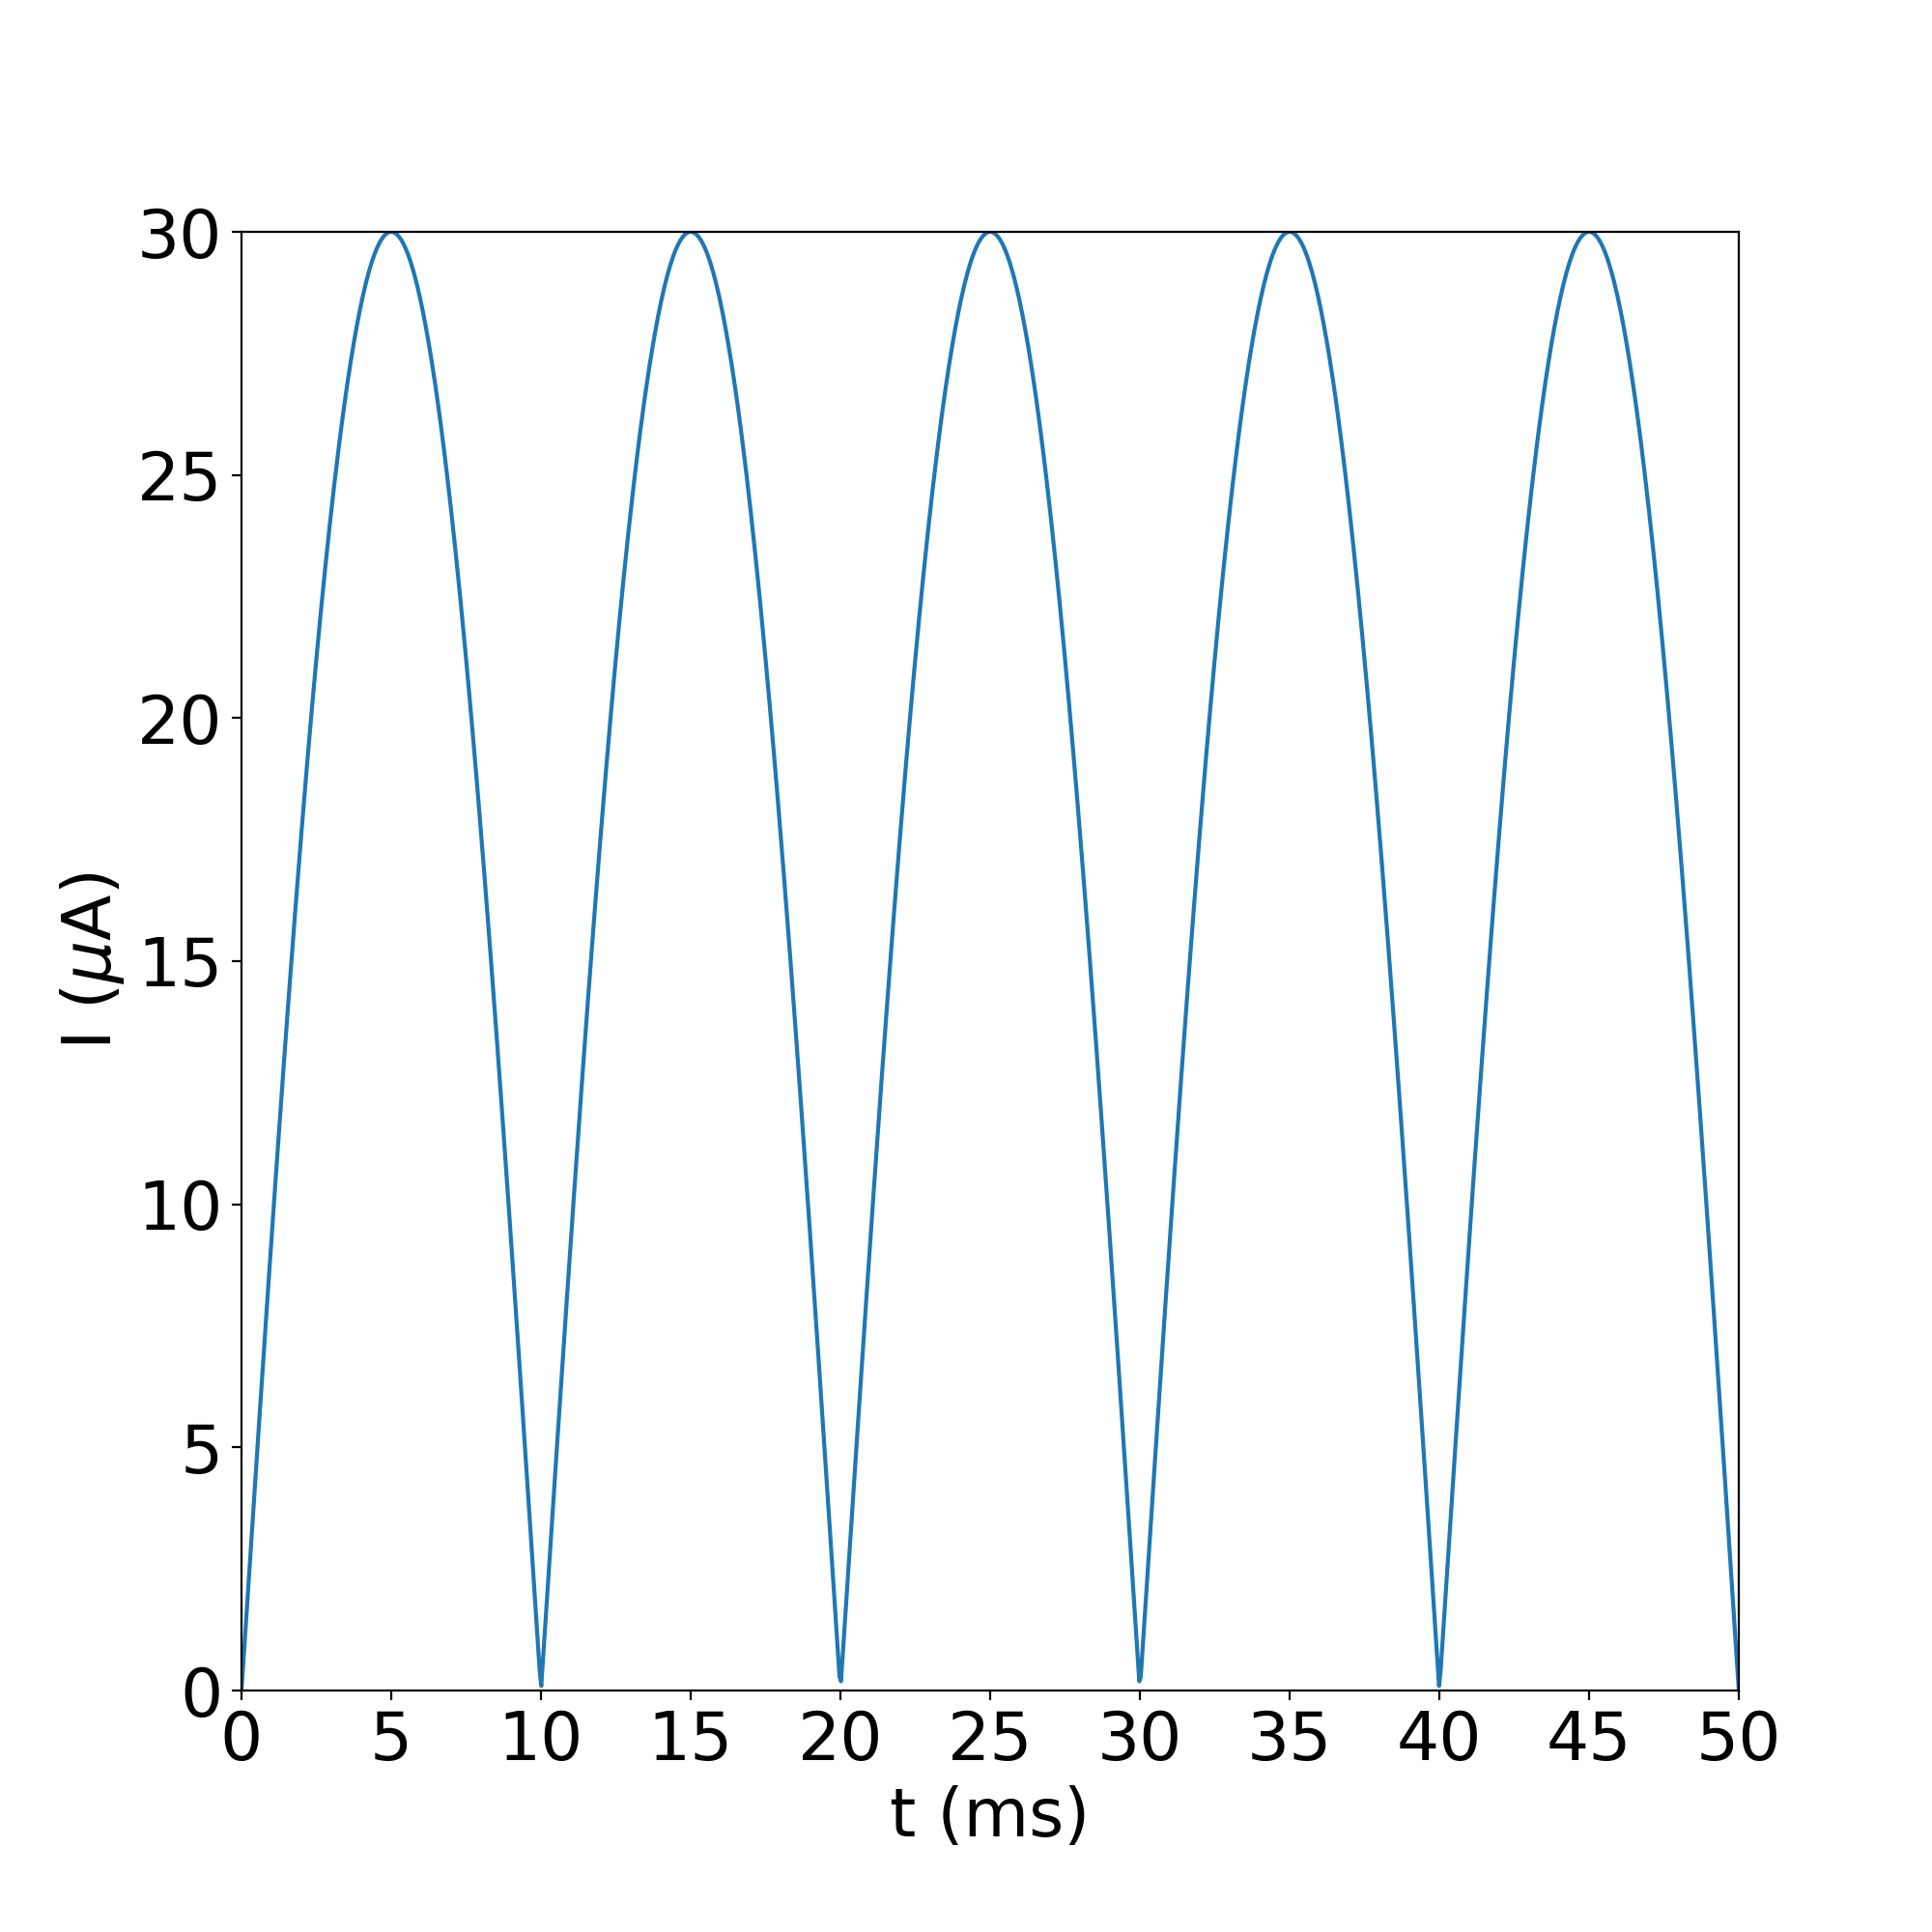
\includegraphics[scale=0.33]{2_1.png}
	\captionsetup{width=\linewidth}  %choose the with of the caption
	\caption{Rectified Sine with an amplitude of 10 $\mu$A for the model visible in Figure 9}
	\label{subsec_fig2_0} %choose a label, see subsection references
\end{figure*}

\newpage
\subsection{Plots of the stimulated LIF Neuron}

\begin{figure*}[hbpt!]					%start figure-environment
	\centering
	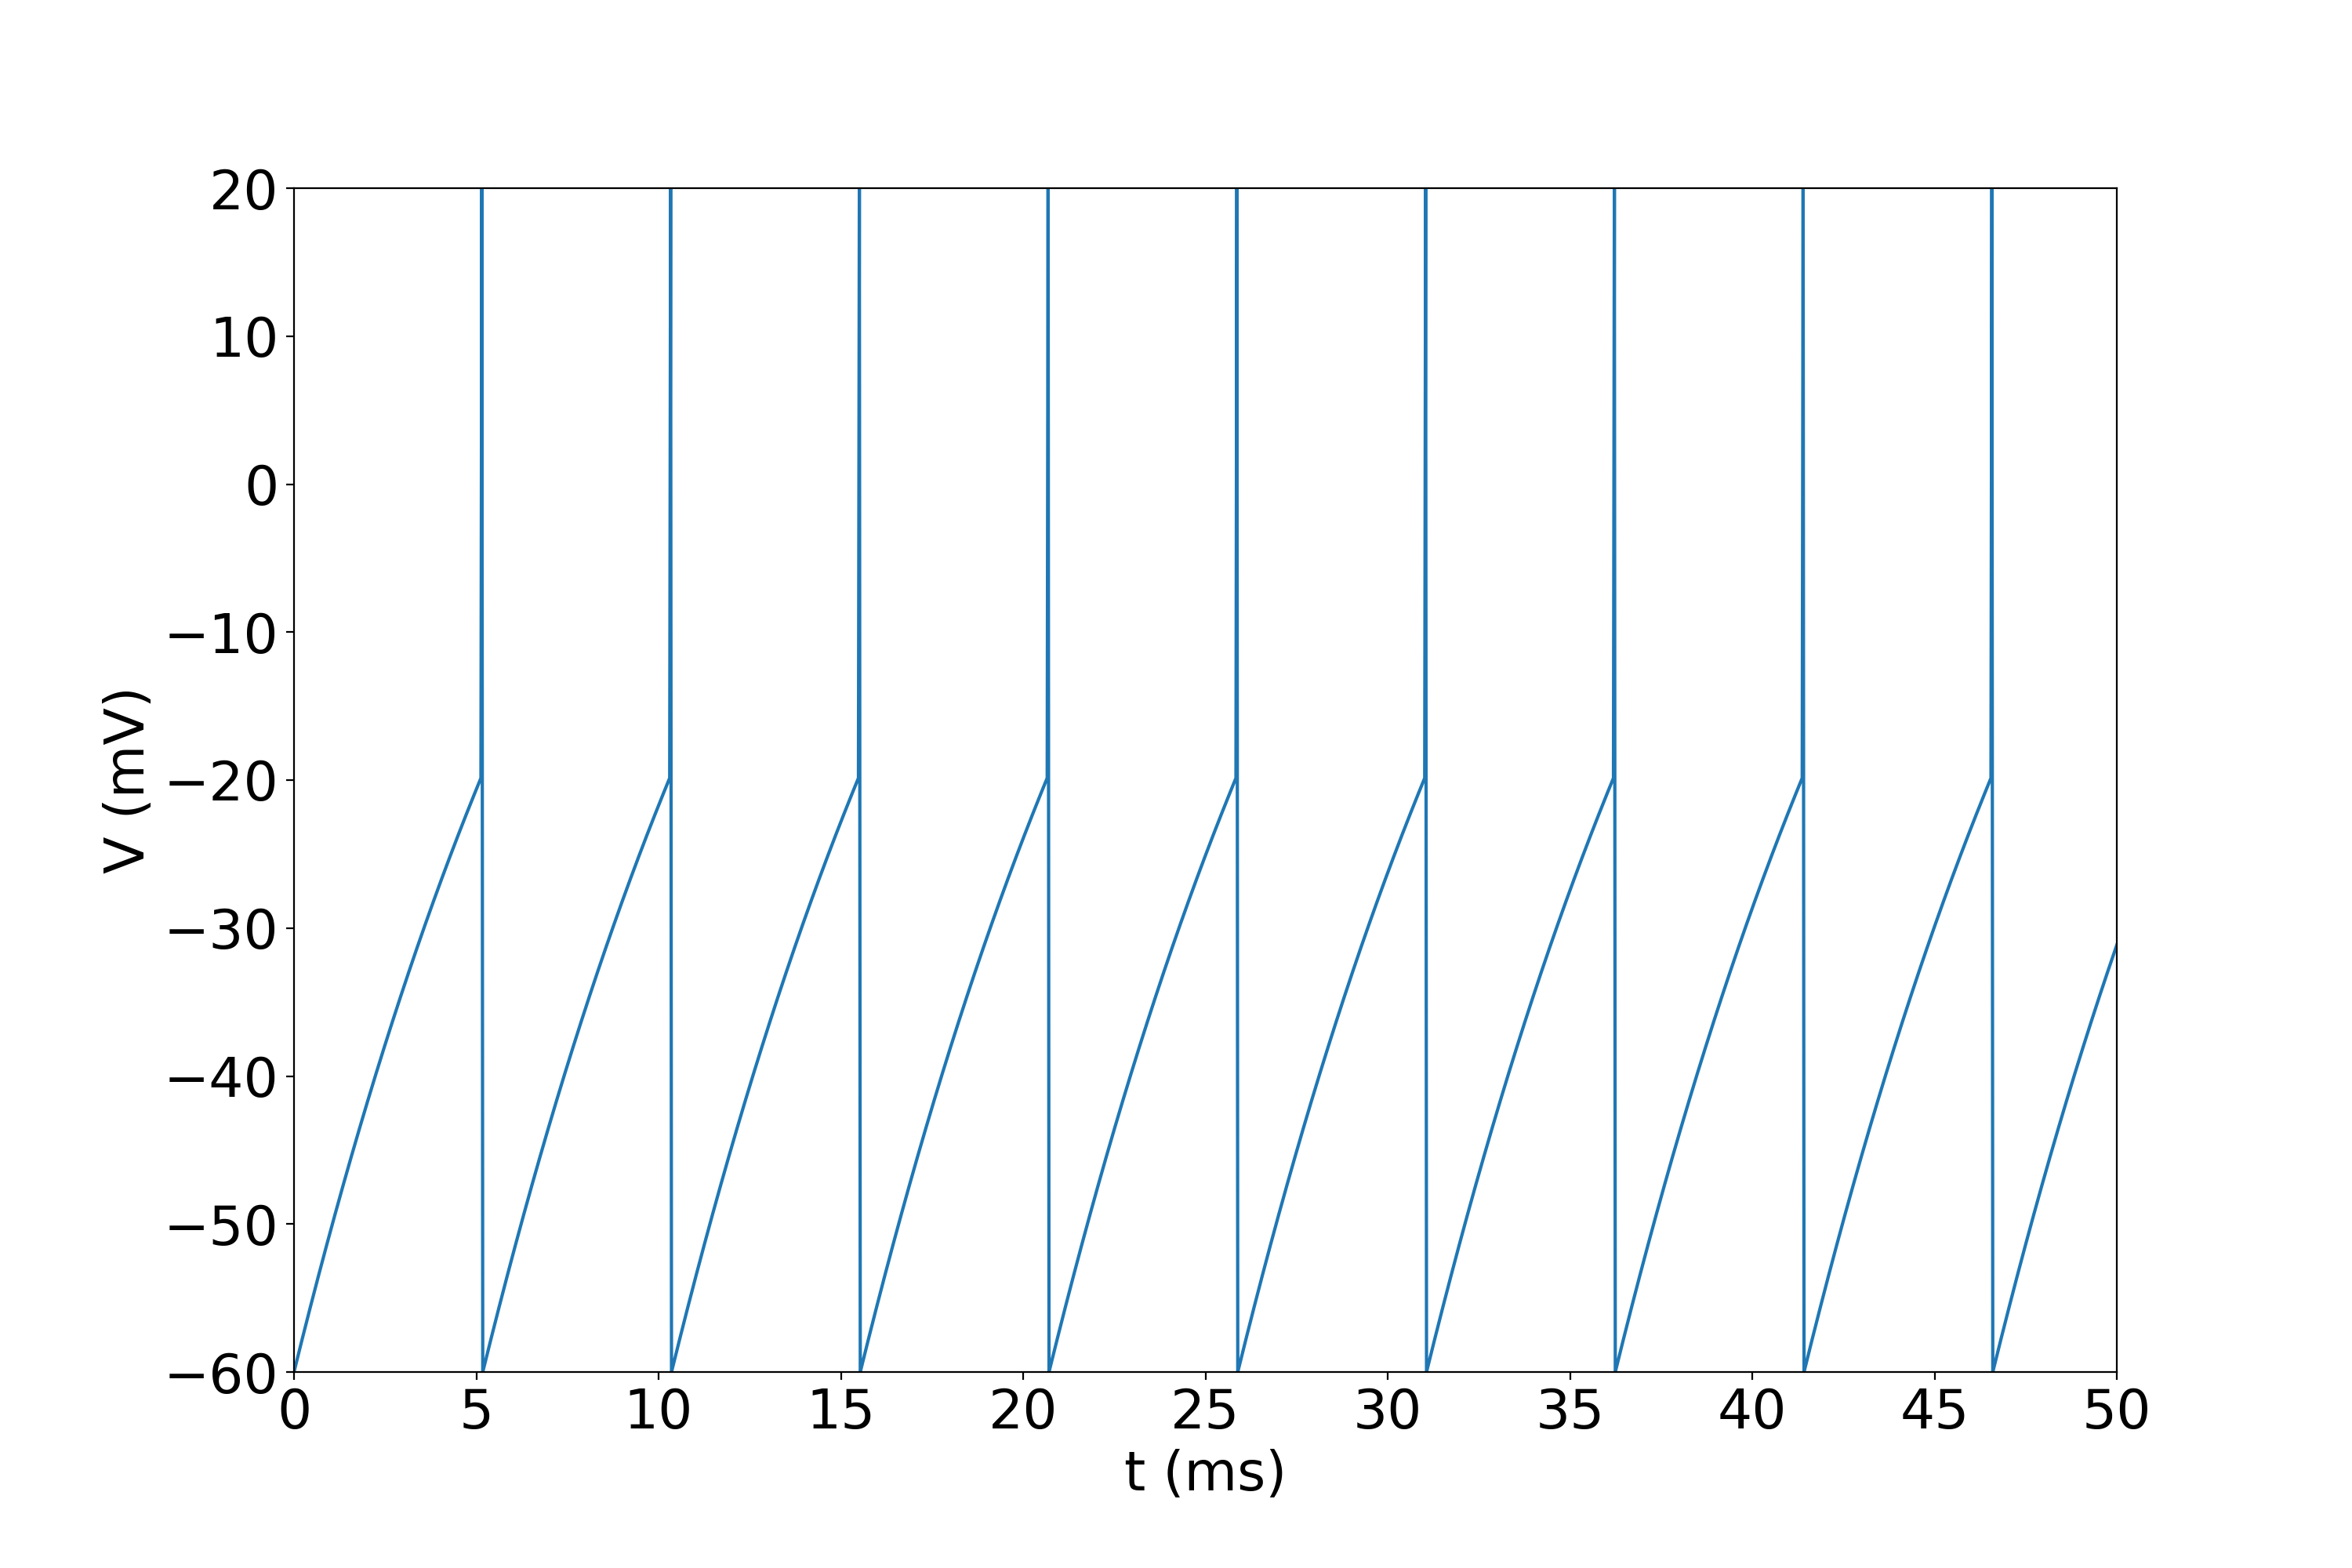
\includegraphics[scale=0.32]{3_1.png}
	\captionsetup{width=\linewidth}  %choose the with of the caption
	\caption{Results for the LIF-Model for different current inputs, for constant current input of 10 $\mu$A}
	\label{subsec_fig2_1} %choose a label, see subsection references
\end{figure*}

\begin{figure*}[hbpt!]					%start figure-environment
	\centering
	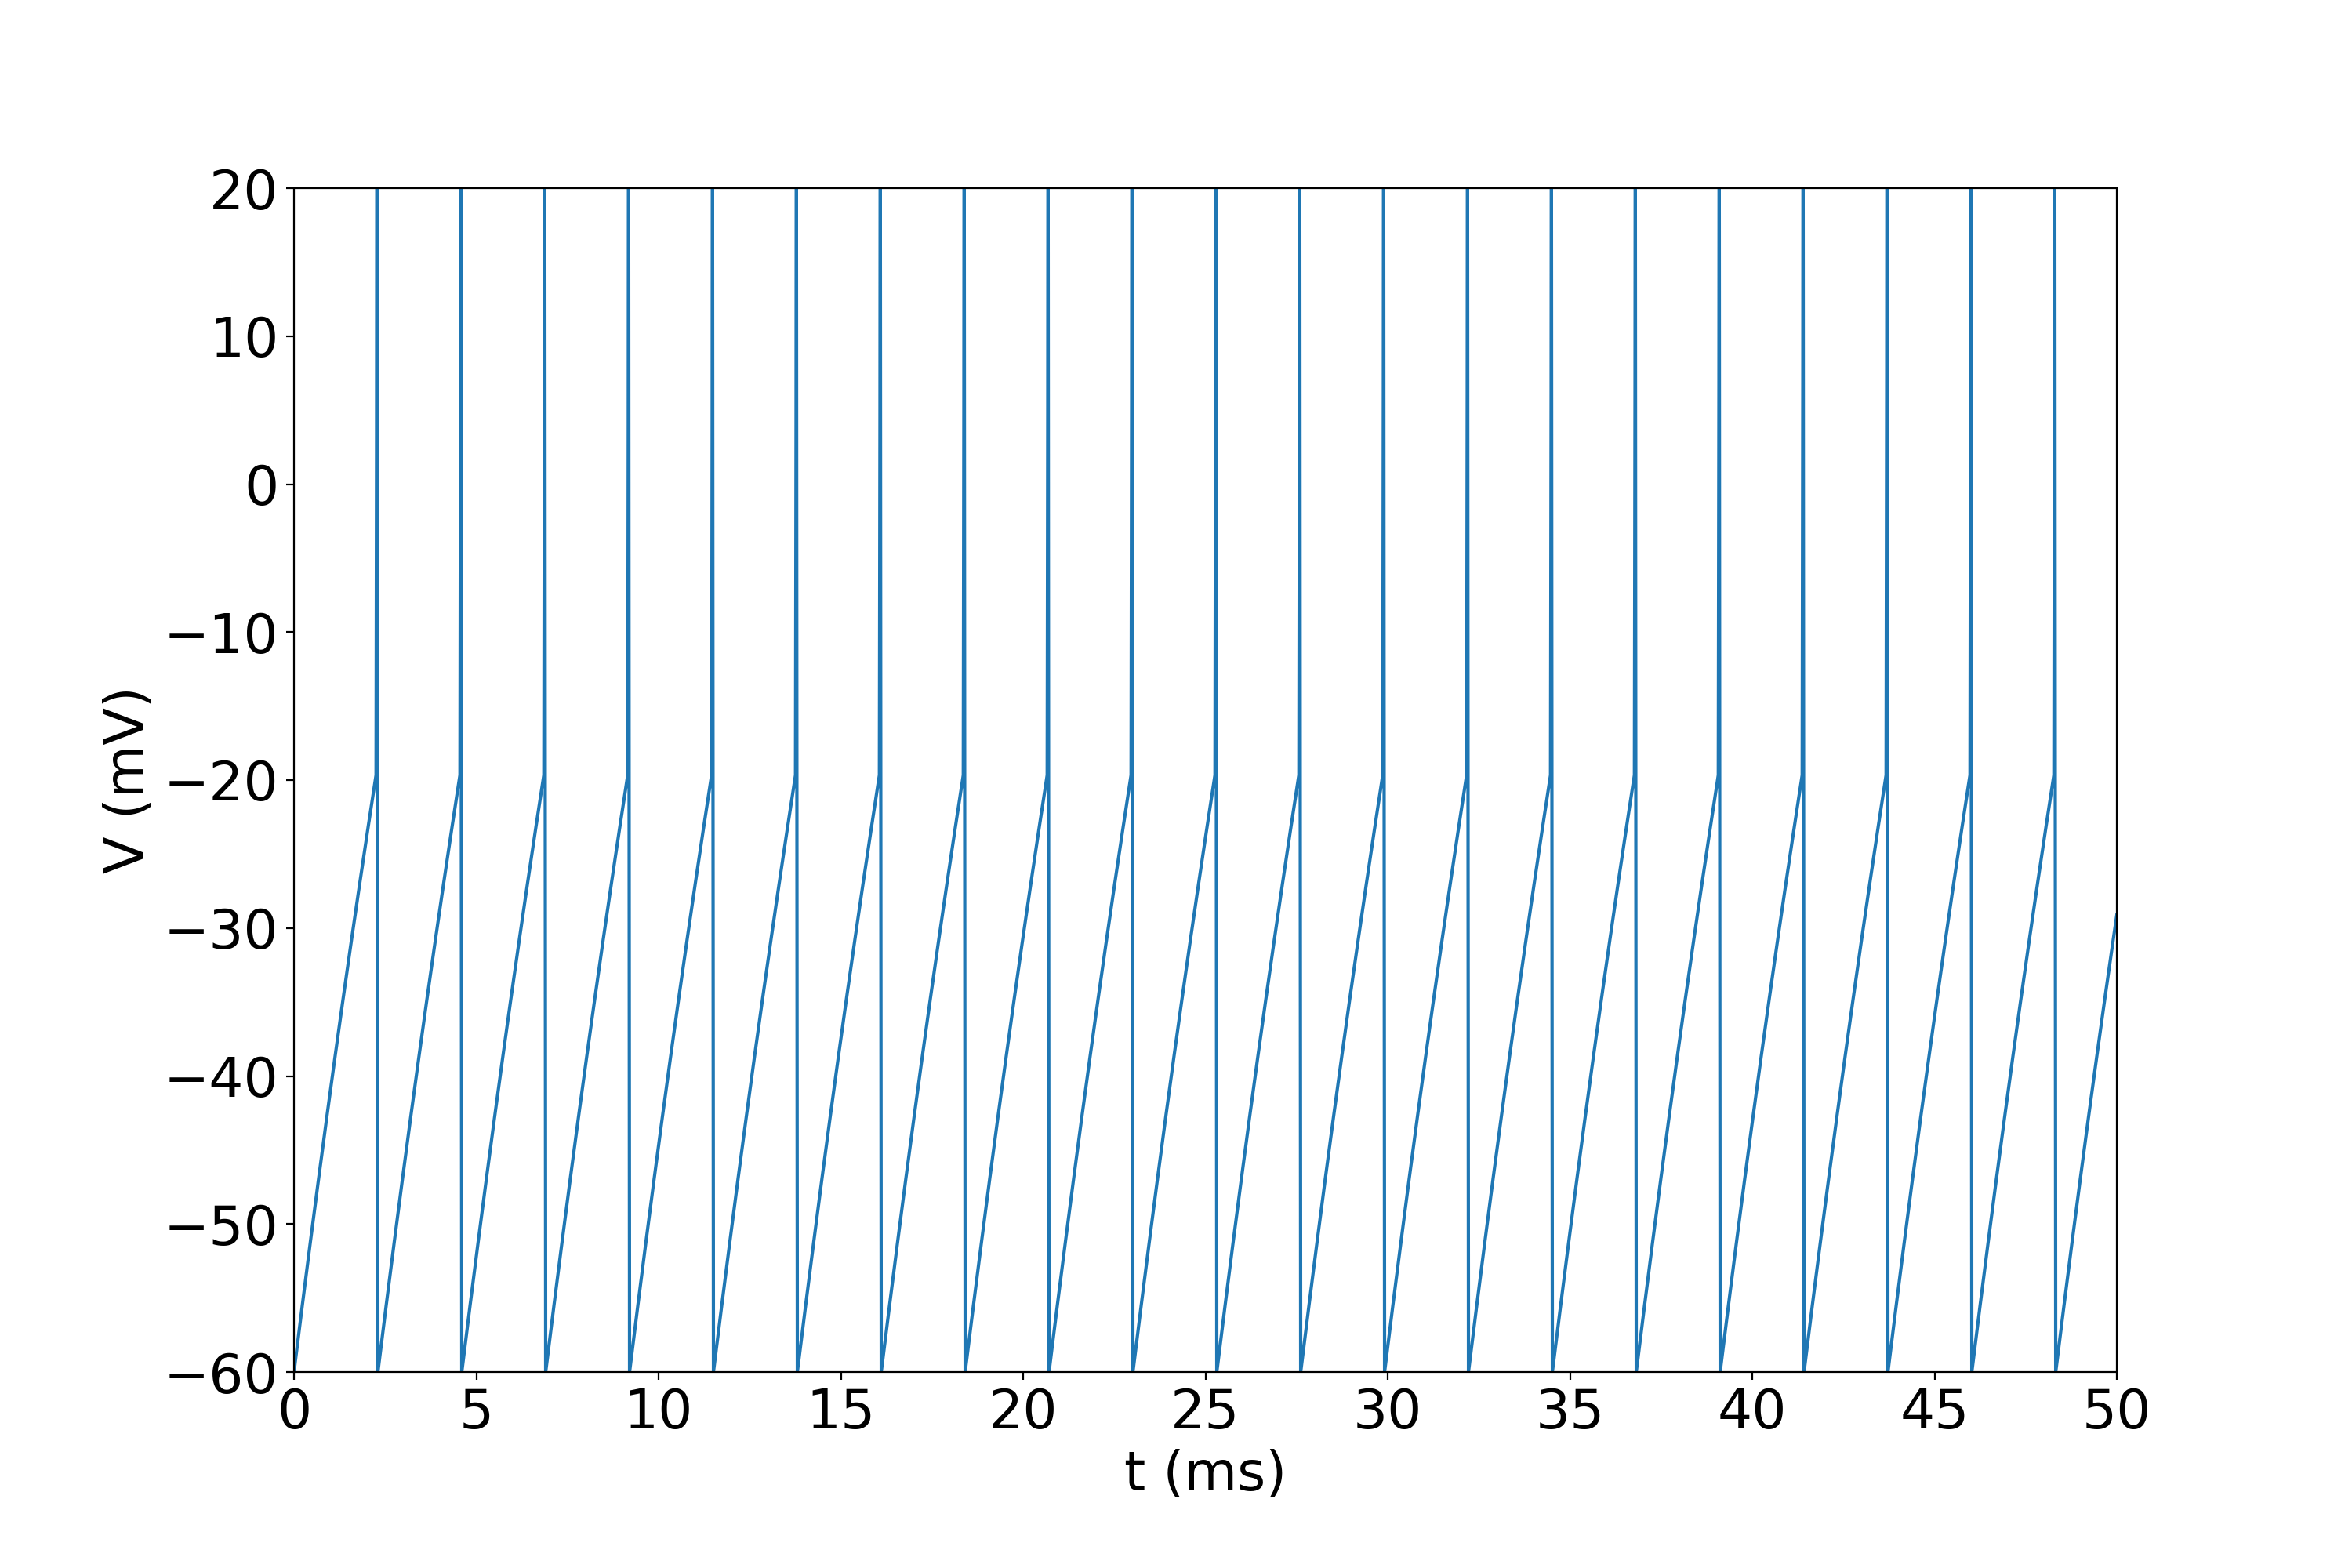
\includegraphics[scale=0.32]{3_2.png}
	\captionsetup{width=\linewidth}  %choose the with of the caption
	\caption{Results for the LIF-Model for different current inputs, for constant current input of 20 $\mu$A}
	\label{subsec_fig2_2} %choose a label, see subsection references
\end{figure*}

\begin{figure*}[hbpt!]					%start figure-environment
	\centering
	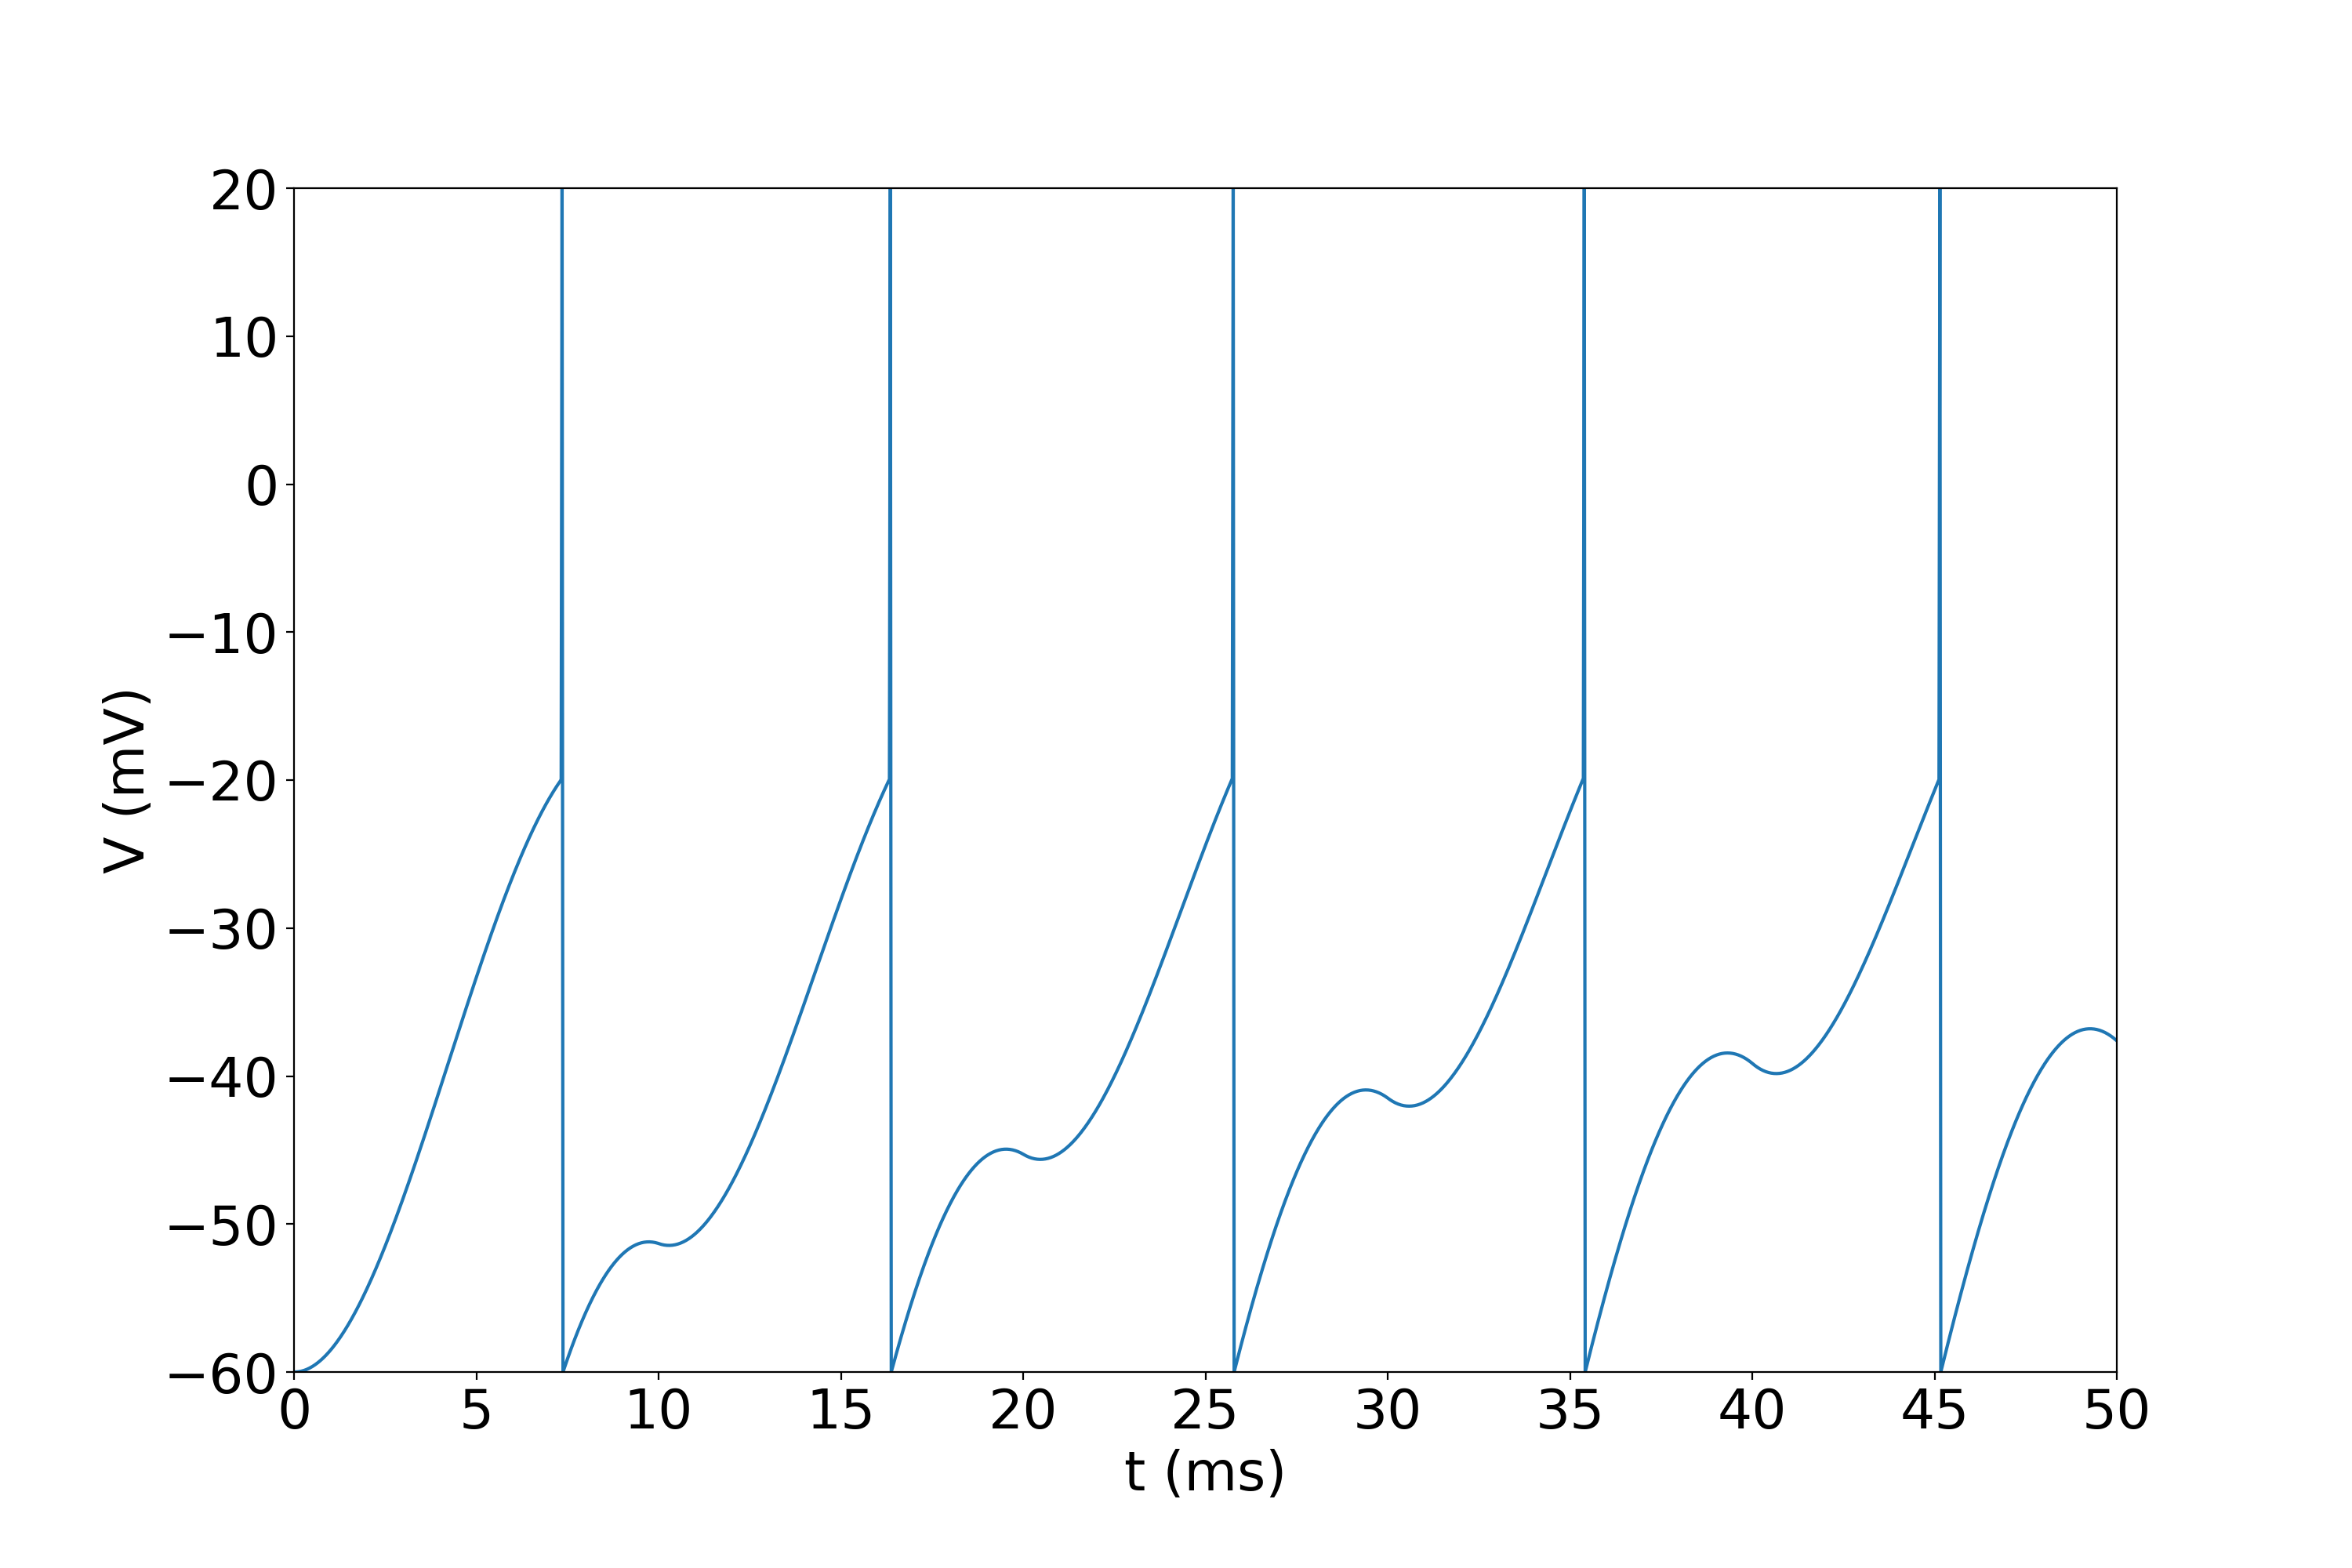
\includegraphics[scale=0.33]{3_3.png}
	\captionsetup{width=\linewidth}  %choose the with of the caption
	\caption{Results for the LIF-Model for different current inputs, for Rectified Sine-Input with an amplitude of 10 $\mu$A, input signal visible in figure 4.}
	\label{subsec_fig2_3} %choose a label, see subsection references
\end{figure*}

\begin{figure*}[h]					%start figure-environment
	\centering
	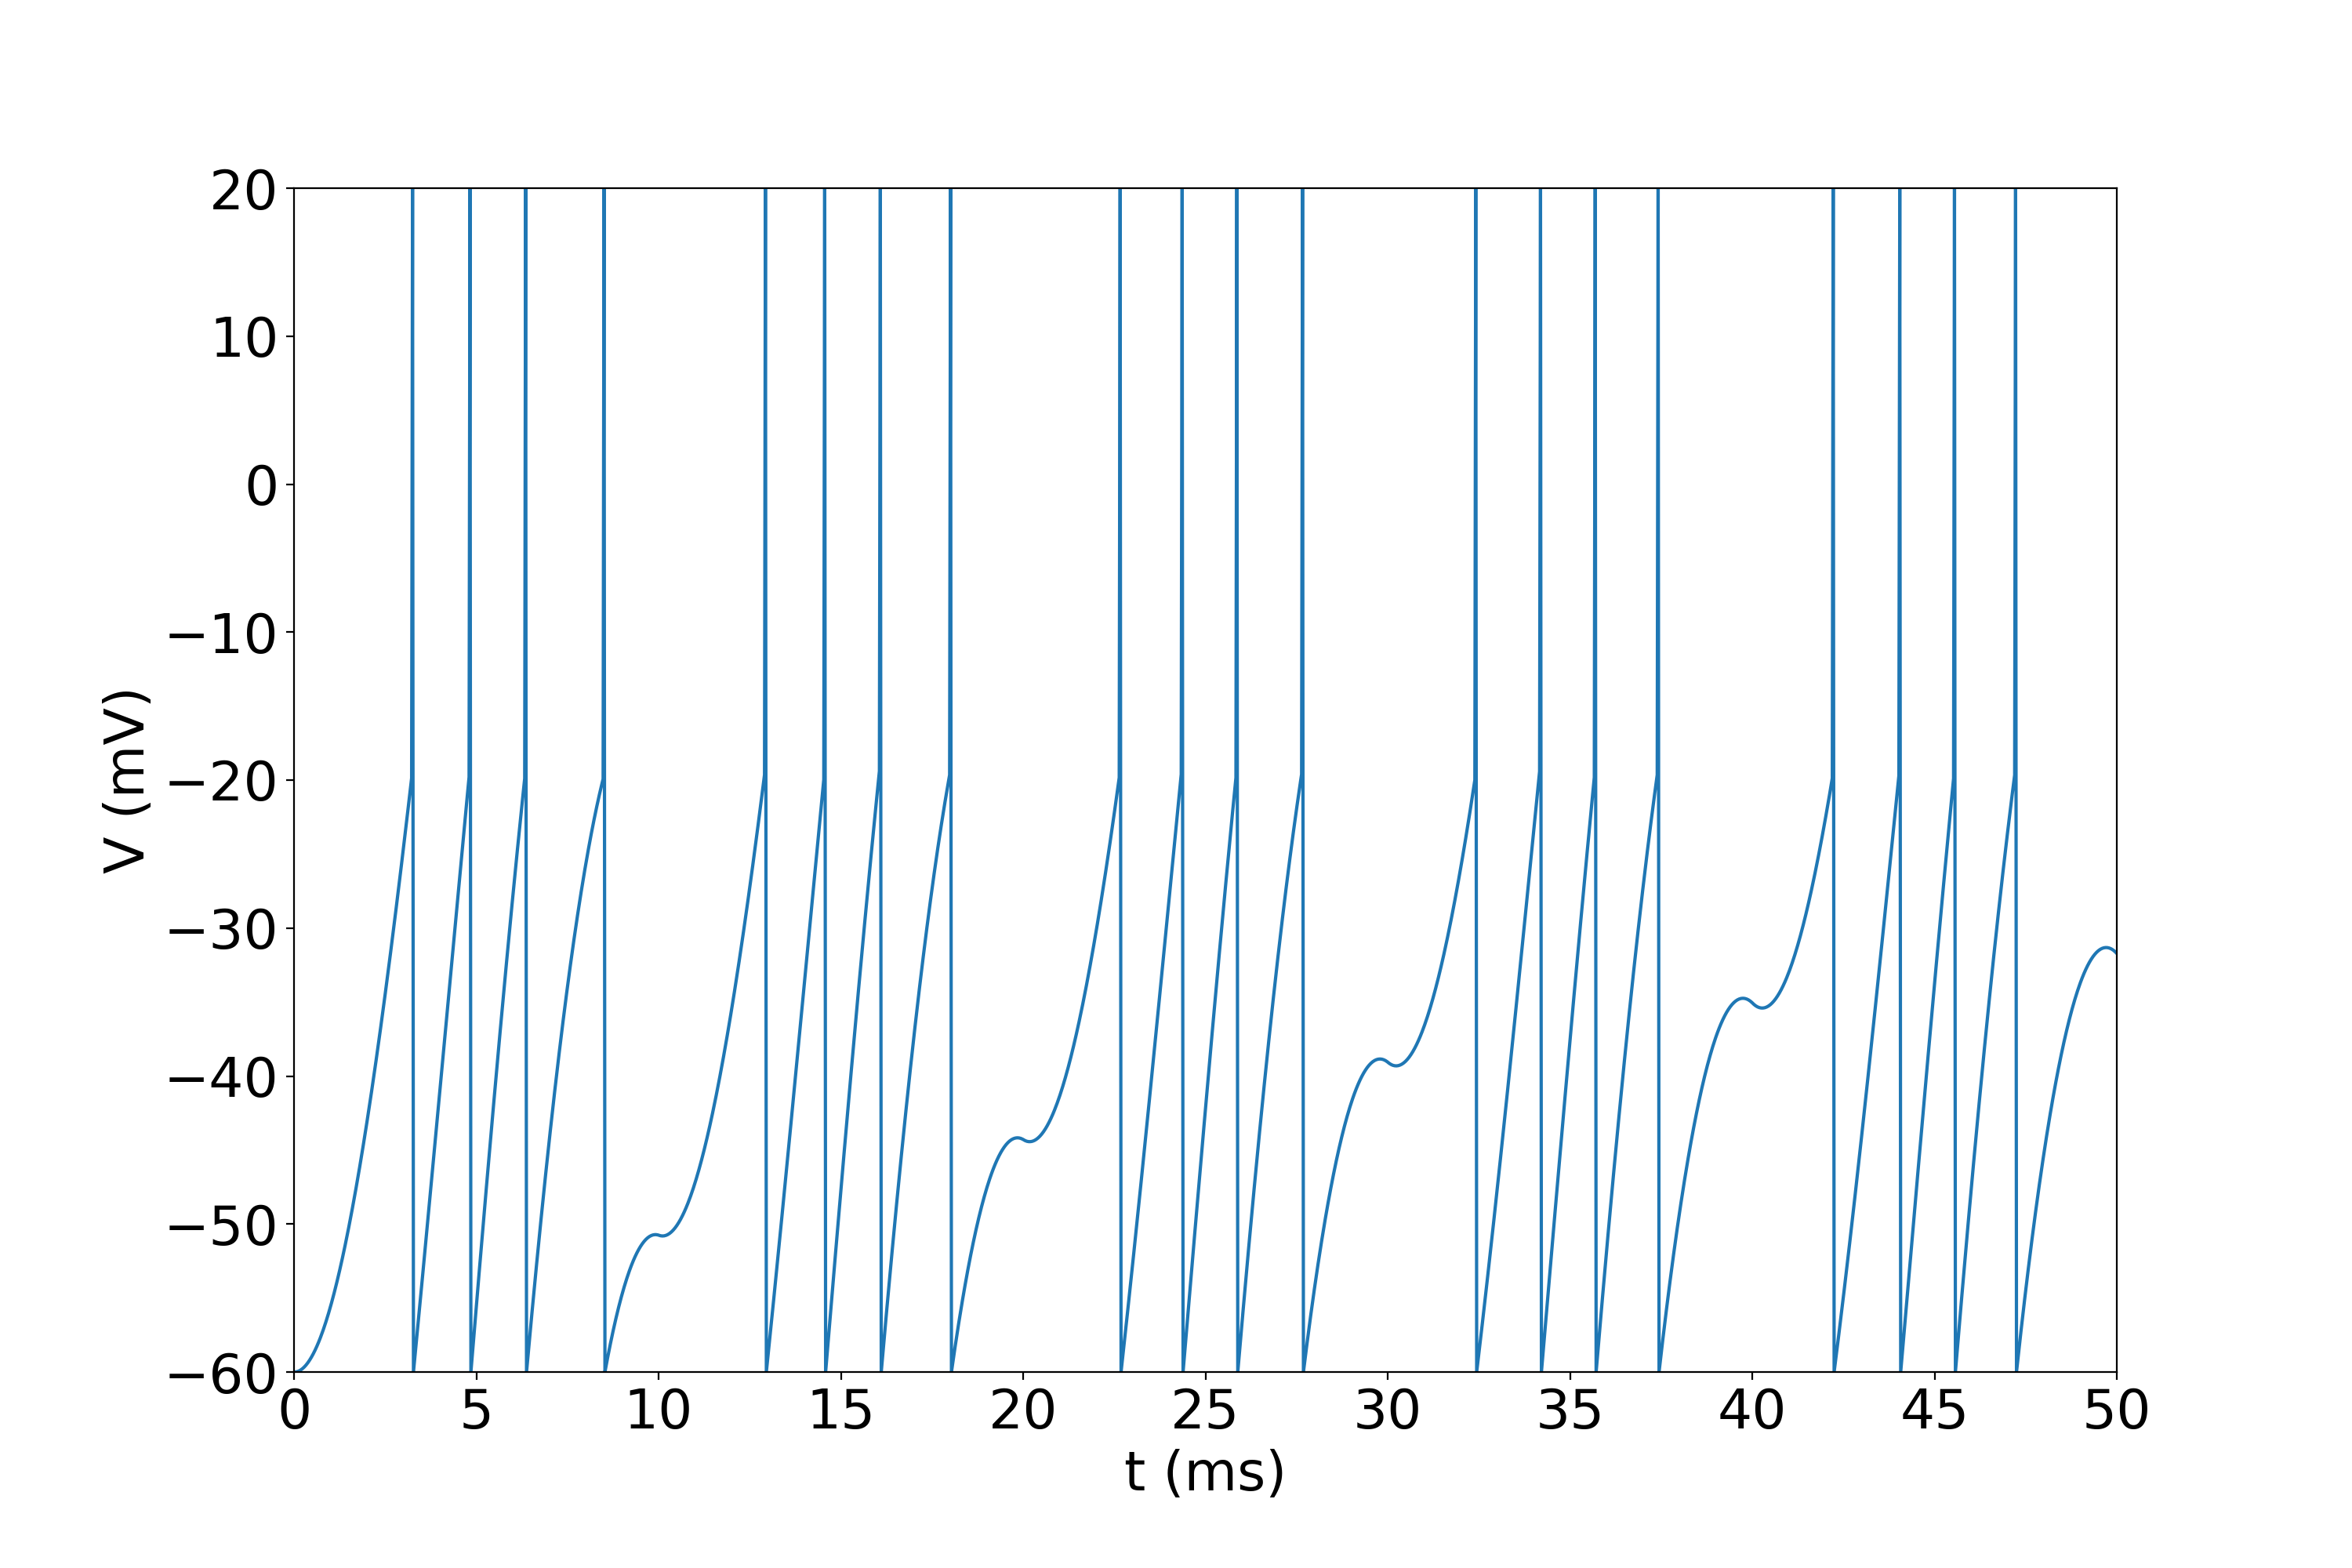
\includegraphics[scale=0.33]{3_4.png}
	\captionsetup{width=\linewidth}  %choose the with of the caption
	\caption{Results for the LIF-Model for different current inputs, for Rectified Sine-Input with an amplitude of 30 $\mu$A, input signal visible in figure 5.}
	\label{subsec_fig2_3} %choose a label, see subsection references
\end{figure*}


\end{document}
